\chapterimage{apps.jpg}

\chapter{Layer 7: Application}

\begin{minipage}{0.4\linewidth}
\begin{center}
\begin{bytefield}{16}
\bitbox{16}{\color{color1} Layer 7: Application} \\
\bitbox{16}{Layer 4: Transport} \\
\bitbox{16}{Layer 3: Internet} \\
\bitbox{16}{Layer 2: Network (LAN)} \\
\bitbox{16}{Layer 1: Physical} \\
\end{bytefield}
\end{center}
\end{minipage}
\begin{minipage}{0.6\linewidth}
\begin{center}
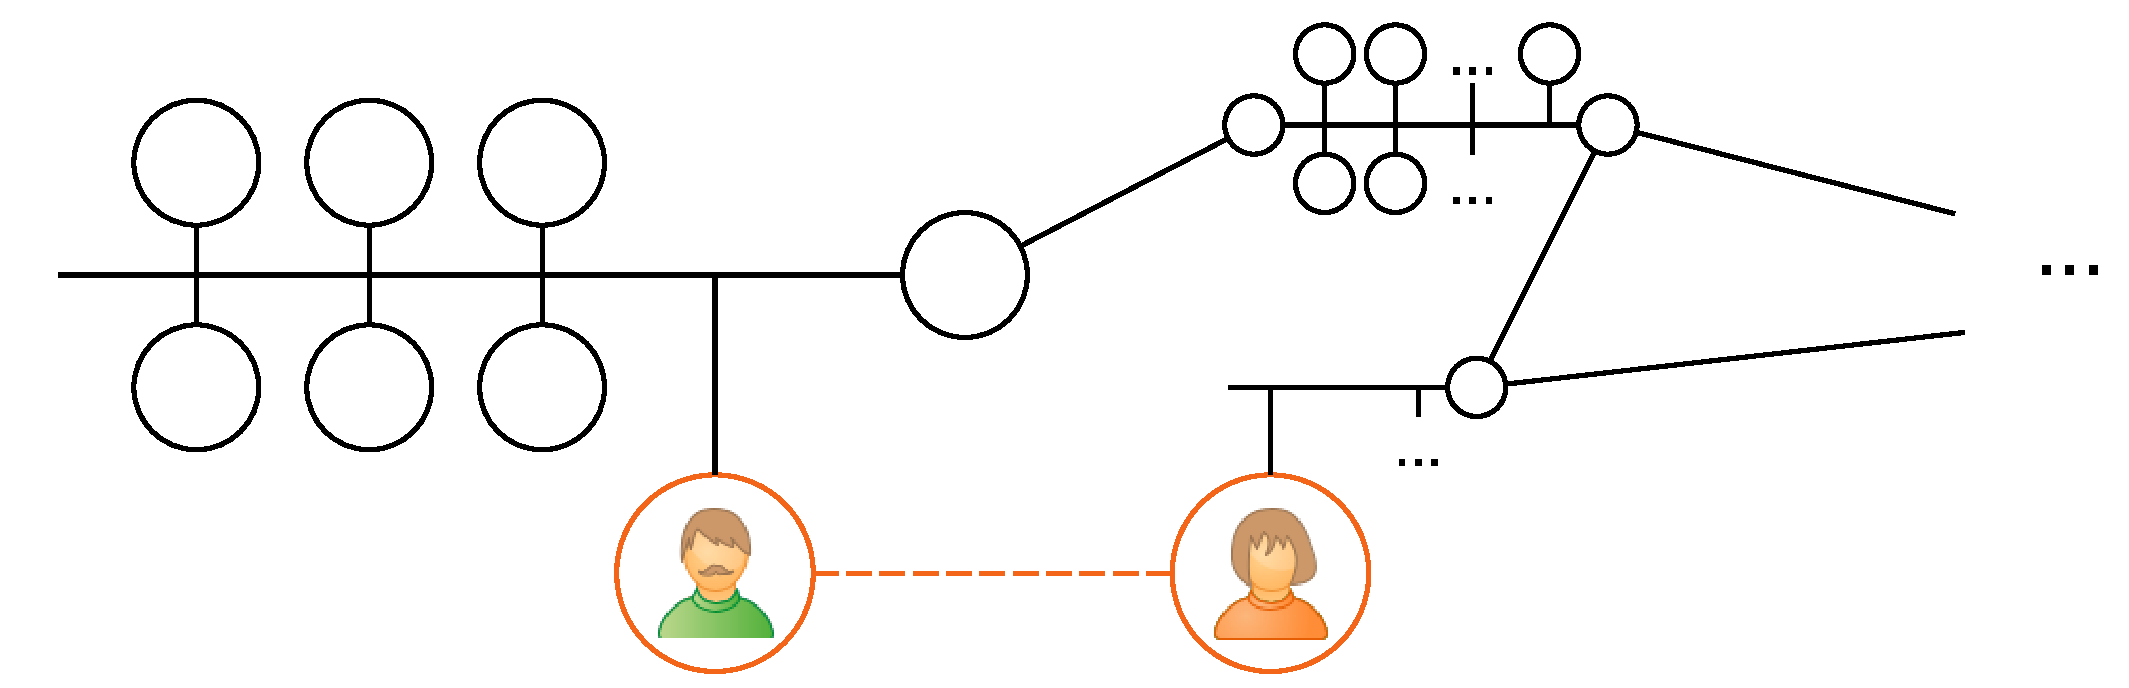
\includegraphics[width=\linewidth]{network_layer7.pdf}
\end{center}
\end{minipage}

The top layer of the TCP/IP network stack includes all applications 
that use TCP or UDP for transport. It is by far the one that contains 
the largest number of protocols, and where those protocols are more 
quickly created and replaced.

In addition to user apps, there are several auxiliary protocols that 
help with configuration and operation issues of virtually 
all internet applications.

\section{DNS -- Domain Name System}

The \concept{DNS} protocol is responsible for translating \conceptRef{domain name}{domain names}
such as \otherBase{ietf.org} or\\\otherBase{cv.uab.cat} into \concept{IP}
addresses that can placed inside \conceptRef{datagram}{datagrams}.

DNS services are run on both \concept{TCP} and \concept{UDP}, \ie, both transport protocols
can be enabled. In both cases, port \otherBase{53} is used.

\subsection{Hierarchy}\label{sec:layer6:dns:hierarchy}

\begin{center}
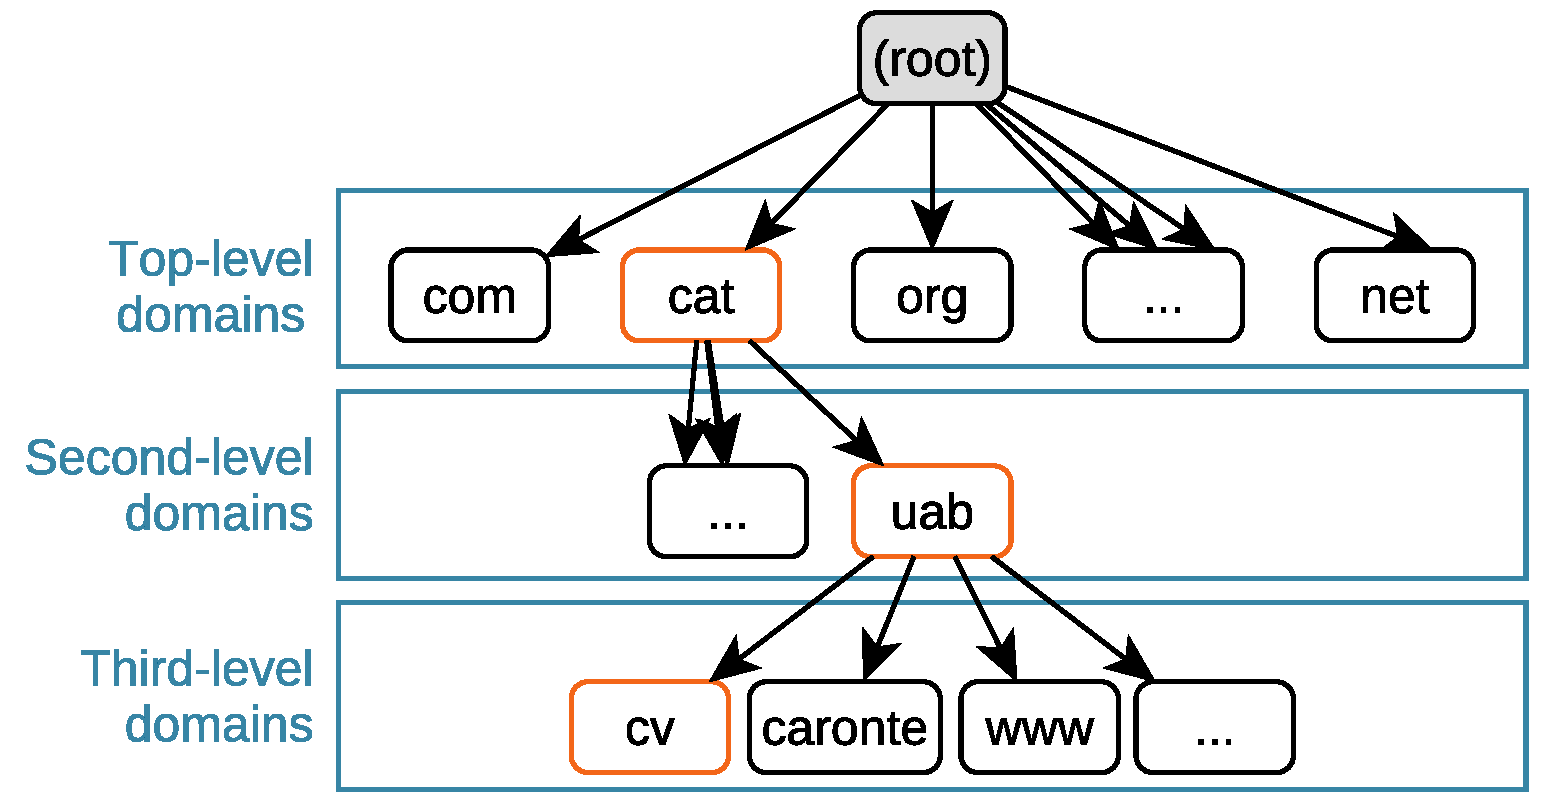
\includegraphics[width=0.65\linewidth]{dns_hierarchy.pdf}
\end{center}

Internet domain names are sequences of names separated by dots. 
These names are presented from the specific to the general in a hierarchical fashion.
For instance, in \otherBase{cv.uab.cat}, \otherBase{cv} belongs to \otherBase{uab.cat},
and \otherBase{uab} to \otherBase{cat}.
% 
The rightmost name, \eg, \otherBase{cat} or \otherBase{com} 
must be one of IANA's \conceptRef{top-level domain}{top-level domains}.

DNS servers are organized in the same hierarchical way as those domain names.
There are $13$ \concept{root DNS} servers (\inlineCode{Root-A} to \inlineCode{Root-M}),
which are responsible for all top-level domains.
You can ask any of them about \otherBase{com}, 
but also about \otherBase{su}, and they will know about them.

That does not mean that any root server knows about every domain \textit{under}
their top-level domain (\eg, \otherBase{uab.cat}): they just know about those 
\href{https://en.wikipedia.org/wiki/List_of_Internet_top-level_domains}{\underline{top-level domains}}.
(\eg, \otherBase{cat}).
% 
The job of the root DNS servers is to redirect you to another DNS server in charge 
of the \concept{top-level domain} you requested.
 
Similarly, the DNS servers responsible for \otherBase{cat} will know about 
any existing \otherBase{*.cat} domain (\eg, \otherBase{uab.cat}), 
but not about subdomains (\eg, \otherBase{cv.uab.cat}). 
% 
The job of those top-level domain DNS servers is to redirect you to 
other DNS servers \concept{authoritative} for the second-level domain 
requested (\eg, \otherBase{uab.cat}).
% 
Second-level domains can then structure their name \concept{zone} 
as desired, including any subdomain number and depth, as well as
the name to IP translation \textit{within} the zone of authority.

\begin{exercise}
Everyone uses DNS all the time. What would be the risks of having
a centralized name translation system instead of DNS's distributed nature.
\end{exercise}

\subsection{Records}

DNS can be seen as a distributed database with different types of entries
called \conceptRef{DNS record}{records}. The main ones are:

\begin{itemize}
\item[\textbf{A}:] An \concept{A} entry maps a domain name to an IPv4 address.
\item[\textbf{AAAA}:] An \concept{AAAA} entry maps a domain name to an IPv6 address.
\item[\textbf{NS}:] An \concept{NS} points to a DNS server that can help.
\item[\textbf{MX}:] A \concept{MX} entry provides the domain name of the email server 
  that handles messages for a domain.
\item[\textbf{CNAME}:] A \concept{CNAME} entry maps a domain name to another domain name.
\end{itemize}

Applications make \conceptRef{request}{requests} to DNS servers indicating the type 
of records they are interested in. Server \conceptRef{reply}{replies} may be for
the requested \concept{A} or \concept{MX} records, 
but the client may also receive a redirection to another DNS (\concept{NS}) 
or an alias to another domain name (\concept{CNAME}).

\subsection{Resolution}

The distributed and hierarchical nature if the DNS database makes it 
sometimes necessary to exchange multiple messages to satisfy a DNS \concept{query}.
 
For instance, Alice may perform a fully \concept{iterative} resolution all on her own.
The first two replies contain an \concept{NS} entry pointing to the next 
DNS server and the IP address of that DNS server, but not the IP address of the 
requested \otherBase{cv.uab.cat}.

\begin{center}
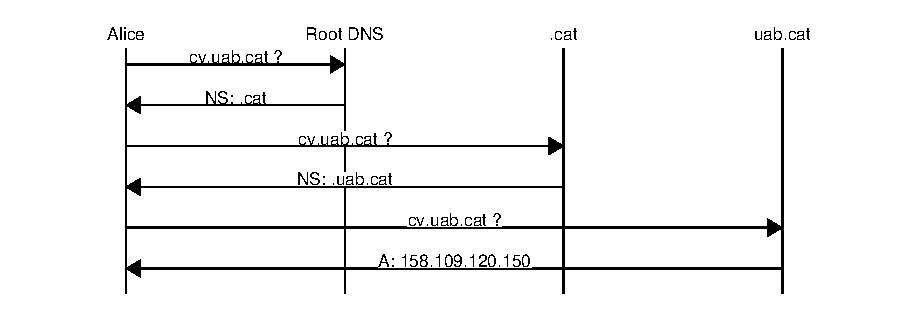
\includegraphics[width=\linewidth]{dns_iterative.eps}
\end{center}

Alice's internet provider (\concept{ISP}) or employer will likely offer DNS servers 
whose job is to receive Alice's requests and resolve them for her in a \concept{recursive} 
manner.

\begin{center}
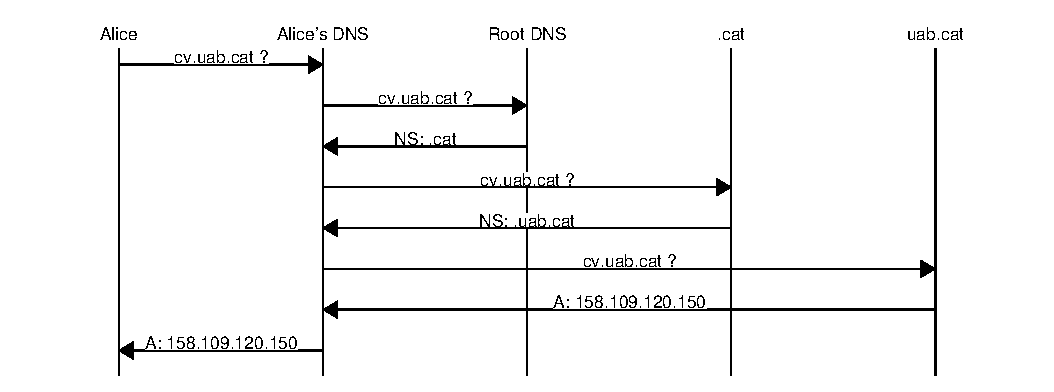
\includegraphics[width=1.05\linewidth]{dns_recursive.eps}
\end{center}

The combination of \concept{recursive} resolution and \concept{cache} tables makes
DNS a pretty efficient system with extremely high availability and low latency.

\begin{exercise}
You can use the \inlineCode{host} and \inlineCode{dig} tools to make DNS queries
and see the results. For instance, my output to \inlineCode{dig uab.cat -t ns}
contains the following lines:

\vspace{0.25cm}
\begin{verbatim}
;; QUESTION SECTION:
;uab.cat.                       IN      NS
;; ANSWER SECTION:
uab.cat.                172800  IN      NS      dns.uab.es.
;; ADDITIONAL SECTION:
dns.uab.es.             172112  IN      A       158.109.0.1
\end{verbatim}
\vspace{0.25cm}

\begin{itemize}
\item What type of record did I request?
\item What two record types did I receive?
\item Why did I receive two record types?
\item Perform a manual iterative resolution of \otherBase{cv.uab.cat}.
  You may start with something like \inlineCode{dig @202.12.27.33 cv.uab.cat}
  to query the M root server.
\end{itemize}


\end{exercise}


- the host utility

% \vspace{-0.75cm}

- DNS
- DHCP
- Application protocols: HTTP, SMTP, IMAP
- AS, rip/ospf

- capas TLS, compresión

% - client vs server (in TCP/IP, symmetry)?
% - server-client model
% - global structure, ownership and organization, 
